% !TeX encoding = UTF-8
% !TeX root = sigmod2018.tex
% !TeX spellcheck = en_US

\vspace{-0.3cm}
\section{Introduction}
\label{sec:Introduction}


The key objective of database systems is to reliably manage data, where high query throughput and low query latency are core requirements~\cite{BeckmanReport2016}. To satisfy these requirements, database systems constantly adapt to novel hardware features~\cite{DBLP:journals/cacm/BonczKM08,DBLP:conf/sigmod/BressFT16,DBLP:conf/sigmod/DoKPPPD13,DBLP:journals/pvldb/KarnagelHL17,DBLP:conf/sigmod/LiDSN16,DBLP:conf/sigmod/OukidLNWL16}. In the recent past, we have seen numerous advances, in particular with respect to \emph{memory}, \emph{processing elements}, and \emph{interconnects}~\cite{DBLP:journals/cacm/BorkarC11,DBLP:journals/dt/Henkel17b,DBLP:conf/micro/Pollack99}. Although it has been intensively studied and commonly accepted that hardware error rates increase dramatically with the decrease of the underlying chip structures ~\cite{DBLP:journals/micro/Borkar05,DBLP:conf/dac/HenkelBDGNSTW13,DBLP:conf/mtdt/SpicaM04}, most database system research activities neglected this fact, traditionally focusing on improving performance characteristics exploiting new data structures and efficient algorithms and leaving error detection (and error correction to some extent) to the underlying hardware. Especially for memory, silent data corruption (SDC) as a result of transient bit flips leading to faulty data is mainly detected and corrected at the DRAM and memory-controller layer~\cite{DBLP:conf/mtdt/SpicaM04}. However, since future hardware becomes less reliable~\cite{DBLP:conf/dac/HenkelBDGNSTW13,DBLP:books/daglib/0037372,DBLP:journals/it/ShafiqueABCCDEH15} and error detection as well as correction by hardware becomes more expensive, this free-ride will come to an end in the near future.

The increasing hardware unreliability is already observable. For instance, repeatedly accessing one memory cell in DRAM modules causes bit flips in physi\-cally-adjacent memory cells~\cite{DBLP:conf/isca/KimDKFLLWLM14,DBLP:conf/date/Mutlu17}. The reason for this is a hardware failure mechanism called \emph{disturbance error}~\cite{DBLP:conf/isca/KimDKFLLWLM14,DBLP:conf/date/Mutlu17}, where electromagnetic (cell-to-cell) interference leads to bit flips. It is already known that this interference effect increases with smaller feature sizes and higher densities of transistors~\cite{DBLP:conf/isca/KimDKFLLWLM14,DBLP:conf/date/Mutlu17}. Kim et al.~\cite{DBLP:conf/isca/KimDKFLLWLM14} evaluated that all newer DRAM modules are affected and they observed one to four bit flips per $64$ bit word even for error-correcting code DRAM (ECC DRAM). Other recent studies have also shown that multi-bit flips become more frequent and that the bit flip model changes at run-time due to transistor aging~\cite{DBLP:conf/isca/KimDKFLLWLM14,DBLP:books/daglib/0037372}. Additionally, hardware-based protection is very challenging~\cite{DBLP:conf/dac/HenkelBDGNSTW13,DBLP:books/daglib/0037372,DBLP:journals/it/ShafiqueABCCDEH15}. Thus, the semiconductor as well as hardware/software communities have recently experienced a shift towards mitigating these reliability issues also at higher software layers, rather than completely mitigating these issues in hardware~\cite{DBLP:conf/dac/HenkelBDGNSTW13,DBLP:books/daglib/0037372}.

Consequently, several software-level reliability techniques have evolved, e.g., error detection using duplicated instructions~\cite{oh2002error} or software implemented fault tolerance (SWIFT)~\cite{DBLP:conf/cgo/ReisCVRA05}. These general-purpose software techniques are usually based on data/code redundancy using dual or triple modular redundancy (DMR/TMR). However, the application of these techniques with respect to in-memory database systems causes a high overhead as illustrated in Figure~\ref{fig:teaser}. Obviously, software-based DMR protection requires twice as much memory capacity compared to a normal (unprotected) setting, since data must be kept twice in different main memory locations. Furthermore, every query is redundantly executed with an additional voting at the end resulting in a computational overhead slightly higher than 2x. Figure~\ref{fig:teaser} highlights the average relative overheads for all $13$ queries of the SSB benchmark~\cite{oneil2009ssbm,DBLP:journals/corr/Sanchez16a} with the unprotected approach as baseline.

\begin{figure}[t]
	{
		\footnotesize
		\graphicspath{{results/ssb/}}
		\null
		\begin{subfigure}[t]{1in}
			% GNUPLOT: LaTeX picture with Postscript
\begingroup
  \makeatletter
  \providecommand\color[2][]{%
    \GenericError{(gnuplot) \space\space\space\@spaces}{%
      Package color not loaded in conjunction with
      terminal option `colourtext'%
    }{See the gnuplot documentation for explanation.%
    }{Either use 'blacktext' in gnuplot or load the package
      color.sty in LaTeX.}%
    \renewcommand\color[2][]{}%
  }%
  \providecommand\includegraphics[2][]{%
    \GenericError{(gnuplot) \space\space\space\@spaces}{%
      Package graphicx or graphics not loaded%
    }{See the gnuplot documentation for explanation.%
    }{The gnuplot epslatex terminal needs graphicx.sty or graphics.sty.}%
    \renewcommand\includegraphics[2][]{}%
  }%
  \providecommand\rotatebox[2]{#2}%
  \@ifundefined{ifGPcolor}{%
    \newif\ifGPcolor
    \GPcolortrue
  }{}%
  \@ifundefined{ifGPblacktext}{%
    \newif\ifGPblacktext
    \GPblacktexttrue
  }{}%
  % define a \g@addto@macro without @ in the name:
  \let\gplgaddtomacro\g@addto@macro
  % define empty templates for all commands taking text:
  \gdef\gplbacktext{}%
  \gdef\gplfronttext{}%
  \makeatother
  \ifGPblacktext
    % no textcolor at all
    \def\colorrgb#1{}%
    \def\colorgray#1{}%
  \else
    % gray or color?
    \ifGPcolor
      \def\colorrgb#1{\color[rgb]{#1}}%
      \def\colorgray#1{\color[gray]{#1}}%
      \expandafter\def\csname LTw\endcsname{\color{white}}%
      \expandafter\def\csname LTb\endcsname{\color{black}}%
      \expandafter\def\csname LTa\endcsname{\color{black}}%
      \expandafter\def\csname LT0\endcsname{\color[rgb]{1,0,0}}%
      \expandafter\def\csname LT1\endcsname{\color[rgb]{0,1,0}}%
      \expandafter\def\csname LT2\endcsname{\color[rgb]{0,0,1}}%
      \expandafter\def\csname LT3\endcsname{\color[rgb]{1,0,1}}%
      \expandafter\def\csname LT4\endcsname{\color[rgb]{0,1,1}}%
      \expandafter\def\csname LT5\endcsname{\color[rgb]{1,1,0}}%
      \expandafter\def\csname LT6\endcsname{\color[rgb]{0,0,0}}%
      \expandafter\def\csname LT7\endcsname{\color[rgb]{1,0.3,0}}%
      \expandafter\def\csname LT8\endcsname{\color[rgb]{0.5,0.5,0.5}}%
    \else
      % gray
      \def\colorrgb#1{\color{black}}%
      \def\colorgray#1{\color[gray]{#1}}%
      \expandafter\def\csname LTw\endcsname{\color{white}}%
      \expandafter\def\csname LTb\endcsname{\color{black}}%
      \expandafter\def\csname LTa\endcsname{\color{black}}%
      \expandafter\def\csname LT0\endcsname{\color{black}}%
      \expandafter\def\csname LT1\endcsname{\color{black}}%
      \expandafter\def\csname LT2\endcsname{\color{black}}%
      \expandafter\def\csname LT3\endcsname{\color{black}}%
      \expandafter\def\csname LT4\endcsname{\color{black}}%
      \expandafter\def\csname LT5\endcsname{\color{black}}%
      \expandafter\def\csname LT6\endcsname{\color{black}}%
      \expandafter\def\csname LT7\endcsname{\color{black}}%
      \expandafter\def\csname LT8\endcsname{\color{black}}%
    \fi
  \fi
    \setlength{\unitlength}{0.0500bp}%
    \ifx\gptboxheight\undefined%
      \newlength{\gptboxheight}%
      \newlength{\gptboxwidth}%
      \newsavebox{\gptboxtext}%
    \fi%
    \setlength{\fboxrule}{0.5pt}%
    \setlength{\fboxsep}{1pt}%
\begin{picture}(1440.00,1440.00)%
    \gplgaddtomacro\gplbacktext{%
      \csname LTb\endcsname%
      \put(448,124){\makebox(0,0)[r]{\strut{}\num{0}}}%
      \csname LTb\endcsname%
      \put(448,375){\makebox(0,0)[r]{\strut{}\num{0.5}}}%
      \csname LTb\endcsname%
      \put(448,625){\makebox(0,0)[r]{\strut{}\num{1}}}%
      \csname LTb\endcsname%
      \put(448,876){\makebox(0,0)[r]{\strut{}\num{1.5}}}%
      \csname LTb\endcsname%
      \put(448,1126){\makebox(0,0)[r]{\strut{}\num{2}}}%
      \csname LTb\endcsname%
      \put(448,1377){\makebox(0,0)[r]{\strut{}\num{2.5}}}%
      \csname LTb\endcsname%
      \put(814,751){\makebox(0,0)[l]{\strut{}1}}%
      \csname LTb\endcsname%
      \put(960,1252){\makebox(0,0)[l]{\strut{}2.01}}%
      \csname LTb\endcsname%
      \put(1139,826){\makebox(0,0)[l]{\strut{}1.19}}%
    }%
    \gplgaddtomacro\gplfronttext{%
      \csname LTb\endcsname%
      \put(130,750){\rotatebox{-270}{\makebox(0,0){\strut{}Relative Runtime}}}%
    }%
    \gplbacktext
    \put(0,0){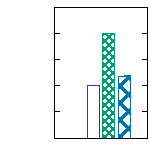
\includegraphics{runtimes}}%
    \gplfronttext
  \end{picture}%
\endgroup

			%\caption{Runtime}
			\caption{Runtime}
			\label{fig:teaser:runtime}%
		\end{subfigure}
		\hfill
		\begin{subfigure}[t]{1in}
			% GNUPLOT: LaTeX picture with Postscript
\begingroup
  \makeatletter
  \providecommand\color[2][]{%
    \GenericError{(gnuplot) \space\space\space\@spaces}{%
      Package color not loaded in conjunction with
      terminal option `colourtext'%
    }{See the gnuplot documentation for explanation.%
    }{Either use 'blacktext' in gnuplot or load the package
      color.sty in LaTeX.}%
    \renewcommand\color[2][]{}%
  }%
  \providecommand\includegraphics[2][]{%
    \GenericError{(gnuplot) \space\space\space\@spaces}{%
      Package graphicx or graphics not loaded%
    }{See the gnuplot documentation for explanation.%
    }{The gnuplot epslatex terminal needs graphicx.sty or graphics.sty.}%
    \renewcommand\includegraphics[2][]{}%
  }%
  \providecommand\rotatebox[2]{#2}%
  \@ifundefined{ifGPcolor}{%
    \newif\ifGPcolor
    \GPcolortrue
  }{}%
  \@ifundefined{ifGPblacktext}{%
    \newif\ifGPblacktext
    \GPblacktexttrue
  }{}%
  % define a \g@addto@macro without @ in the name:
  \let\gplgaddtomacro\g@addto@macro
  % define empty templates for all commands taking text:
  \gdef\gplbacktext{}%
  \gdef\gplfronttext{}%
  \makeatother
  \ifGPblacktext
    % no textcolor at all
    \def\colorrgb#1{}%
    \def\colorgray#1{}%
  \else
    % gray or color?
    \ifGPcolor
      \def\colorrgb#1{\color[rgb]{#1}}%
      \def\colorgray#1{\color[gray]{#1}}%
      \expandafter\def\csname LTw\endcsname{\color{white}}%
      \expandafter\def\csname LTb\endcsname{\color{black}}%
      \expandafter\def\csname LTa\endcsname{\color{black}}%
      \expandafter\def\csname LT0\endcsname{\color[rgb]{1,0,0}}%
      \expandafter\def\csname LT1\endcsname{\color[rgb]{0,1,0}}%
      \expandafter\def\csname LT2\endcsname{\color[rgb]{0,0,1}}%
      \expandafter\def\csname LT3\endcsname{\color[rgb]{1,0,1}}%
      \expandafter\def\csname LT4\endcsname{\color[rgb]{0,1,1}}%
      \expandafter\def\csname LT5\endcsname{\color[rgb]{1,1,0}}%
      \expandafter\def\csname LT6\endcsname{\color[rgb]{0,0,0}}%
      \expandafter\def\csname LT7\endcsname{\color[rgb]{1,0.3,0}}%
      \expandafter\def\csname LT8\endcsname{\color[rgb]{0.5,0.5,0.5}}%
    \else
      % gray
      \def\colorrgb#1{\color{black}}%
      \def\colorgray#1{\color[gray]{#1}}%
      \expandafter\def\csname LTw\endcsname{\color{white}}%
      \expandafter\def\csname LTb\endcsname{\color{black}}%
      \expandafter\def\csname LTa\endcsname{\color{black}}%
      \expandafter\def\csname LT0\endcsname{\color{black}}%
      \expandafter\def\csname LT1\endcsname{\color{black}}%
      \expandafter\def\csname LT2\endcsname{\color{black}}%
      \expandafter\def\csname LT3\endcsname{\color{black}}%
      \expandafter\def\csname LT4\endcsname{\color{black}}%
      \expandafter\def\csname LT5\endcsname{\color{black}}%
      \expandafter\def\csname LT6\endcsname{\color{black}}%
      \expandafter\def\csname LT7\endcsname{\color{black}}%
      \expandafter\def\csname LT8\endcsname{\color{black}}%
    \fi
  \fi
    \setlength{\unitlength}{0.0500bp}%
    \ifx\gptboxheight\undefined%
      \newlength{\gptboxheight}%
      \newlength{\gptboxwidth}%
      \newsavebox{\gptboxtext}%
    \fi%
    \setlength{\fboxrule}{0.5pt}%
    \setlength{\fboxsep}{1pt}%
\begin{picture}(1440.00,1440.00)%
    \gplgaddtomacro\gplbacktext{%
      \csname LTb\endcsname%
      \put(448,124){\makebox(0,0)[r]{\strut{}\num{0}}}%
      \csname LTb\endcsname%
      \put(448,375){\makebox(0,0)[r]{\strut{}\num{0.5}}}%
      \csname LTb\endcsname%
      \put(448,625){\makebox(0,0)[r]{\strut{}\num{1}}}%
      \csname LTb\endcsname%
      \put(448,876){\makebox(0,0)[r]{\strut{}\num{1.5}}}%
      \csname LTb\endcsname%
      \put(448,1126){\makebox(0,0)[r]{\strut{}\num{2}}}%
      \csname LTb\endcsname%
      \put(448,1377){\makebox(0,0)[r]{\strut{}\num{2.5}}}%
      \csname LTb\endcsname%
      \put(814,751){\makebox(0,0)[l]{\strut{}1}}%
      \csname LTb\endcsname%
      \put(960,1252){\makebox(0,0)[l]{\strut{}2.00}}%
      \csname LTb\endcsname%
      \put(1139,1001){\makebox(0,0)[l]{\strut{}1.50}}%
    }%
    \gplgaddtomacro\gplfronttext{%
      \csname LTb\endcsname%
      \put(6,750){\rotatebox{-270}{\makebox(0,0){\strut{}Relative Memory}}}%
      \put(130,750){\rotatebox{-270}{\makebox(0,0){\strut{}Consumption}}}%
    }%
    \gplbacktext
    \put(0,0){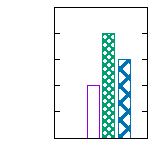
\includegraphics{consumption}}%
    \gplfronttext
  \end{picture}%
\endgroup

			%\caption{Memory Consumption}
			\caption{Storage}
			\label{fig:teaser:memory}%
		\end{subfigure}
		\hfill
		\begin{subfigure}[t]{0.8in}
			% GNUPLOT: LaTeX picture with Postscript
\begingroup
  \makeatletter
  \providecommand\color[2][]{%
    \GenericError{(gnuplot) \space\space\space\@spaces}{%
      Package color not loaded in conjunction with
      terminal option `colourtext'%
    }{See the gnuplot documentation for explanation.%
    }{Either use 'blacktext' in gnuplot or load the package
      color.sty in LaTeX.}%
    \renewcommand\color[2][]{}%
  }%
  \providecommand\includegraphics[2][]{%
    \GenericError{(gnuplot) \space\space\space\@spaces}{%
      Package graphicx or graphics not loaded%
    }{See the gnuplot documentation for explanation.%
    }{The gnuplot epslatex terminal needs graphicx.sty or graphics.sty.}%
    \renewcommand\includegraphics[2][]{}%
  }%
  \providecommand\rotatebox[2]{#2}%
  \@ifundefined{ifGPcolor}{%
    \newif\ifGPcolor
    \GPcolortrue
  }{}%
  \@ifundefined{ifGPblacktext}{%
    \newif\ifGPblacktext
    \GPblacktexttrue
  }{}%
  % define a \g@addto@macro without @ in the name:
  \let\gplgaddtomacro\g@addto@macro
  % define empty templates for all commands taking text:
  \gdef\gplbacktext{}%
  \gdef\gplfronttext{}%
  \makeatother
  \ifGPblacktext
    % no textcolor at all
    \def\colorrgb#1{}%
    \def\colorgray#1{}%
  \else
    % gray or color?
    \ifGPcolor
      \def\colorrgb#1{\color[rgb]{#1}}%
      \def\colorgray#1{\color[gray]{#1}}%
      \expandafter\def\csname LTw\endcsname{\color{white}}%
      \expandafter\def\csname LTb\endcsname{\color{black}}%
      \expandafter\def\csname LTa\endcsname{\color{black}}%
      \expandafter\def\csname LT0\endcsname{\color[rgb]{1,0,0}}%
      \expandafter\def\csname LT1\endcsname{\color[rgb]{0,1,0}}%
      \expandafter\def\csname LT2\endcsname{\color[rgb]{0,0,1}}%
      \expandafter\def\csname LT3\endcsname{\color[rgb]{1,0,1}}%
      \expandafter\def\csname LT4\endcsname{\color[rgb]{0,1,1}}%
      \expandafter\def\csname LT5\endcsname{\color[rgb]{1,1,0}}%
      \expandafter\def\csname LT6\endcsname{\color[rgb]{0,0,0}}%
      \expandafter\def\csname LT7\endcsname{\color[rgb]{1,0.3,0}}%
      \expandafter\def\csname LT8\endcsname{\color[rgb]{0.5,0.5,0.5}}%
    \else
      % gray
      \def\colorrgb#1{\color{black}}%
      \def\colorgray#1{\color[gray]{#1}}%
      \expandafter\def\csname LTw\endcsname{\color{white}}%
      \expandafter\def\csname LTb\endcsname{\color{black}}%
      \expandafter\def\csname LTa\endcsname{\color{black}}%
      \expandafter\def\csname LT0\endcsname{\color{black}}%
      \expandafter\def\csname LT1\endcsname{\color{black}}%
      \expandafter\def\csname LT2\endcsname{\color{black}}%
      \expandafter\def\csname LT3\endcsname{\color{black}}%
      \expandafter\def\csname LT4\endcsname{\color{black}}%
      \expandafter\def\csname LT5\endcsname{\color{black}}%
      \expandafter\def\csname LT6\endcsname{\color{black}}%
      \expandafter\def\csname LT7\endcsname{\color{black}}%
      \expandafter\def\csname LT8\endcsname{\color{black}}%
    \fi
  \fi
    \setlength{\unitlength}{0.0500bp}%
    \ifx\gptboxheight\undefined%
      \newlength{\gptboxheight}%
      \newlength{\gptboxwidth}%
      \newsavebox{\gptboxtext}%
    \fi%
    \setlength{\fboxrule}{0.5pt}%
    \setlength{\fboxsep}{1pt}%
\begin{picture}(1140.00,1440.00)%
    \gplgaddtomacro\gplbacktext{%
    }%
    \gplgaddtomacro\gplfronttext{%
      \csname LTb\endcsname%
      \put(642,1056){\makebox(0,0)[r]{\strut{}Unprotected}}%
      \csname LTb\endcsname%
      \put(642,750){\makebox(0,0)[r]{\strut{}DMR}}%
      \csname LTb\endcsname%
      \put(642,444){\makebox(0,0)[r]{\strut{}AHEAD}}%
    }%
    \gplbacktext
    \put(0,0){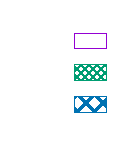
\includegraphics{legend}}%
    \gplfronttext
  \end{picture}%
\endgroup

		\end{subfigure}
		\null
	}
	\vspace{-0.2cm}
%	\caption{Comparing the unprotected in-memory database concept with protected concepts of double modular redundancy (DMR) and our \emph{AHEAD} approach using the star-schema benchmark~\cite{DBLP:journals/corr/Sanchez16a}. More details in Section~\ref{sec:SSBEval}.}
\caption{Relative comparison using the star-schema benchmark~\cite{DBLP:journals/corr/Sanchez16a}. More details in Section~\ref{sec:SSBEval}.}
	\label{fig:teaser}
	\vspace{-0.5cm}
\end{figure}

\textbf{Core Contribution.}
Generally, any undetected bit flip destroys the reliability objective of database systems in form of false negatives (missing tuples), false positives (tuples with invalid predicates) or inaccurate aggregates in a silent way. Since (i) general-purpose software-based protection techniques introduce too much overhead, (ii) memory systems will be significantly more error-prone in the future due to smaller chip structures, and (iii) generic hardware-level detection mechanisms will be too costly and too inflexible, there is a clear need for database-specific approaches to guarantee reliable data storage and processing without sacrificing the overall performance. In this paper, we present a novel approach called \emph{AHEAD} for \textbf{error detection} tailored to state-of-the-art in-memory column store systems~\cite{DBLP:journals/debu/IdreosGNMMK12,DBLP:conf/vldb/StonebrakerABCCFLLMOORTZ05}. As highlighted in Figure~\ref{fig:teaser}, our \emph{AHEAD} approach reduces the overhead compared to DMR to a large degree for storage as well as for processing. Furthermore, multi-bit flips occurring during query processing are on-the-fly detectable, which is not the case for DMR, where errors are only detected during the voting at the end~\cite{DBLP:conf/isca/ReinhardtM00}. We achieve this property and the significant overhead reduction by encoding each value in a fine-grained way using a software-based error coding scheme, which allows to directly work on the encoded data representation during query processing. Moreover, we intentionally devise an \textbf{error detection}-only mechanism and leave the repair mechanism to the database system itself, e.g. by deploying a fine-grained recovery procedure. We intentionally also position our approach \textbf{orthogonal} to other coding domains like compression~\cite{DBLP:conf/sigmod/AbadiMF06} or encryption~\cite{DBLP:journals/sigmod/ShmueliVEG09}, which allows a free combination of different schemes to the underlying data. To represent the intention of detecting hardware errors, we introduce new terms for encoding and decoding. We denote the process of encoding data as \textbf{data hardening}, since data is literally firmed so that corruption becomes detectable. In contrast, we denote as \textbf{data softening} the decoding of data, as it becomes vulnerable to corruption again. Furthermore, we introduce the notion of \textbf{bit flip weight} as the number of flipped bits per logical data value. 


\textbf{Contributions in Detail and Outline.}
To present our novel \emph{AHEAD} approach in detail, we make the following contributions:  
\begin{compactenum}
	\item Reliability concerns for future hardware have attracted major attention in the recent past. In Section~\ref{sec:ProblemEvidence}, we give a precise problem description and define requirements for reliable data management on future hardware.
	\item We promote arithmetic codes as software-based error coding scheme and AN coding as one representative, in Section~\ref{sec:ErrorCoding}. In particular, we justify that AN coding has unique properties with regard to our defined requirements. 	
	\item Based on AN coding, we present our hardened data storage concept for state-of-the-art in-memory column stores in Section~\ref{sec:DataHardening}. Additionally, we describe the adaptation of our hardened storage for various bit flip weights and introduce performance improvements for AN code operations.
	\item Based on this hardened storage foundation, we present our on-the-fly error detection during query processing in Section~\ref{sec:ResilientQueryProcessing}. We introduce different error detection opportunities and determine \emph{continuous detection} as the best solution, for which we describe essential query processing adjustments. 
	\item In Sections~\ref{sec:SSBEval} and~\ref{sec:MicroBenchmarks}, we exhaustively evaluate our \emph{AHEAD} approach, the underlying AN coding scheme, and our developed performance improvements. 
\end{compactenum}
Finally, we present related work in Section~\ref{sec:RelatedWork} as well as briefly summarize the paper including a discussion of future work in Section~\ref{sec:Conclusion}.

